\reportfigure{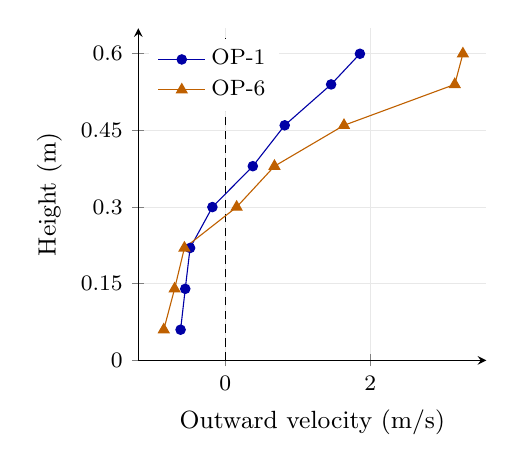
\begin{tikzpicture}
\begin{axis}[width=.495\linewidth,height=5.8cm,axis lines=left,ymin=0,ymax=.65,
ytick={0,.15,.30,.45,.60},xmin=-1.2,xmax=3.6,
xlabel={Outward velocity (m/s)},ylabel={Height (m)},grid=major,grid style={gray!18},
tick label style={font=\footnotesize},label style={font=\small},
legend style={at={(.03,.97)},anchor=north west,font=\footnotesize,draw=none}]
\addplot[black,densely dashed,forget plot] coordinates {(0,0) (0,.63)};
\addplot[blue!65!black,mark=*,mark size=1.7pt] coordinates {(-0.6169,0.06) (-0.5525,0.14) (-0.4858,0.22) (-0.1781,0.3) (0.3791,0.38) (0.8191,0.46) (1.459,0.54) (1.8563,0.6)};
\addlegendentry{OP-1}
\addplot[orange!75!black,mark=triangle*,mark size=2.2pt] coordinates {(-0.8488,0.06) (-0.6996,0.14) (-0.5641,0.22) (0.1562,0.3) (0.6777,0.38) (1.6367,0.46) (3.164,0.54) (3.2764,0.6)};
\addlegendentry{OP-6}
\end{axis}\end{tikzpicture}%
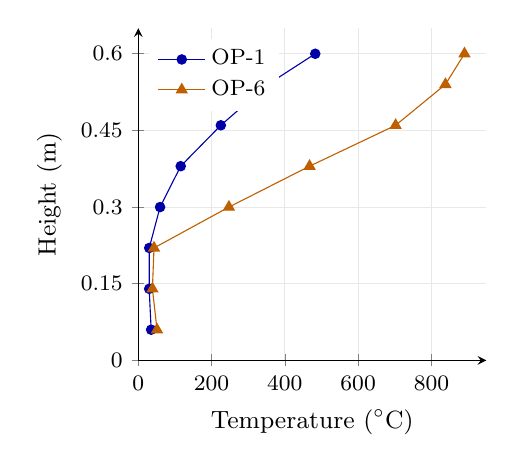
\begin{tikzpicture}
\begin{axis}[width=.495\linewidth,height=5.8cm,axis lines=left,ymin=0,ymax=.65,
ytick={0,.15,.30,.45,.60},xmin=0,xmax=950,
xlabel={Temperature ($^\circ$C)},ylabel={Height (m)},grid=major,grid style={gray!18},
tick label style={font=\footnotesize},label style={font=\small},
legend style={at={(.03,.97)},anchor=north west,font=\footnotesize,draw=none}]

\addplot[blue!65!black,mark=*,mark size=1.7pt] coordinates {(35.0545,0.06) (29.7306,0.14) (29.8055,0.22) (59.4344,0.3) (115.7244,0.38) (225.2291,0.46) (353.3391,0.54) (482.9451,0.6)};
\addlegendentry{OP-1}
\addplot[orange!75!black,mark=triangle*,mark size=2.2pt] coordinates {(51.0932,0.06) (38.5634,0.14) (42.8348,0.22) (247.3595,0.3) (467.4785,0.38) (702.2993,0.46) (838.2762,0.54) (890.311,0.6)};
\addlegendentry{OP-6}
\end{axis}\end{tikzpicture}}{Figure B1. R1 doorway profiles at eight elevations for the adiabatic 106.2~kW diagnostic runs. Each point is a 90--120~s average. Negative velocity denotes incoming air.}
